\chapter{Results}
\label{ch:results}

This chapter presents the results obtained by applying the previously described methods. Due to uncertain normalization
factors, all values are given with respect to the maximum charm component in terms of flux $\dot{\phi}_\nu$ or fluence $\phi_\nu$
as physical quantities. By definition, the flux
\begin{equation*}
	\dot{\phi}_\nu \kern+0.25pt = \frac{d \kern+0.75pt \dot{N}_{\kern-0.5pt \nu} / \kern-1.0pt dE_\nu \kern+0.25pt}{4\pi d^2} \:,
	\label{eqn:flux}
\end{equation*}
counts neutrinos per energy, time and area. This equation derives from evenly spreading all spectral
intensity over a spherical surface with radius equal to the distance $d \kern+0.5pt$ from a single source. Integrating over
time yields the fluence
\begin{equation*}
	\phi_\nu \kern+0.25pt = \frac{dN_{\kern-0.5pt \nu} / \kern-1.0pt dE_\nu \kern+0.25pt}{4\pi d^2} \:,
	\label{eqn:fluence}
\end{equation*}
which measures neutrino numbers per energy and area instead. Because $d \kern+0.5pt$ is a constant, forming ratios of
$\dot{\phi}_\nu$ or $\phi_\nu$ eliminates it. Accordingly, the following results are independent of distance.
As mentioned earlier, neutrinos are not distinguished by their flavor, but by the particle decay from which they
originate. Assuming identical particle and antiparticle population sizes and decay paths, the resulting
factors are absorbed in the normalization, requiring no further consideration. The numerical values provided in Section
\ref{sec:computation} are used for the required model parameters.

Figure \ref{fig:magnetar-charm-comparison-with} shows the temporal evolution of charmed hadron contributions to the
total charm component at $E_\nu = \qty{e9}{\giga\electronvolt}$ originating from a young magnetar.
Decays of $\smash{D^0}$ constitute most of the earlier charmed neutrinos, with $\smash{D^+} \kern-0.5pt$ adding significant amounts
as well, especially at later times. Both $\smash{D^+_s}$ and $\smash{\Lambda^{\kern-0.5pt +}_{\kern+0.5pt c}}$ are roughly
the same, each contributing around \qty{10}{\percent} to the combined flux. This is in line with cross sections calculated
via \eqref{eqn:differential} or measured by \cite{lhc} as well as the respective branching fractions listed in Table
\ref{tab:charm-hadrons} for effective three{\kern+0.3pt}-body decays to neutrinos. Similarly, Figure \ref{fig:magnetar-flux-with}
presents the light curves for pions and kaons in addition to the total charm contribution, restricted to
$\smash{E_\nu = \kern-0.5pt \qty{e9}{\giga\electronvolt}}$ neutrinos. As in \cite{Carpio_2020} from QCD calculations,
a factor ranging from $1 \kern-0.5pt /3$ to $3$ is adopted for the charm hadron uncertainty and highlighted by a shaded blue band. Decays of
kaons generally contribute more than pions at this energy, with neutrinos from charm exceeding both until
$\cramped{t = \kern-0.25pt \qty{e5}{\second}}$ by more than one order of magnitude.

\newpage\null\vfill
\begin{figure}[H]
	\centering
	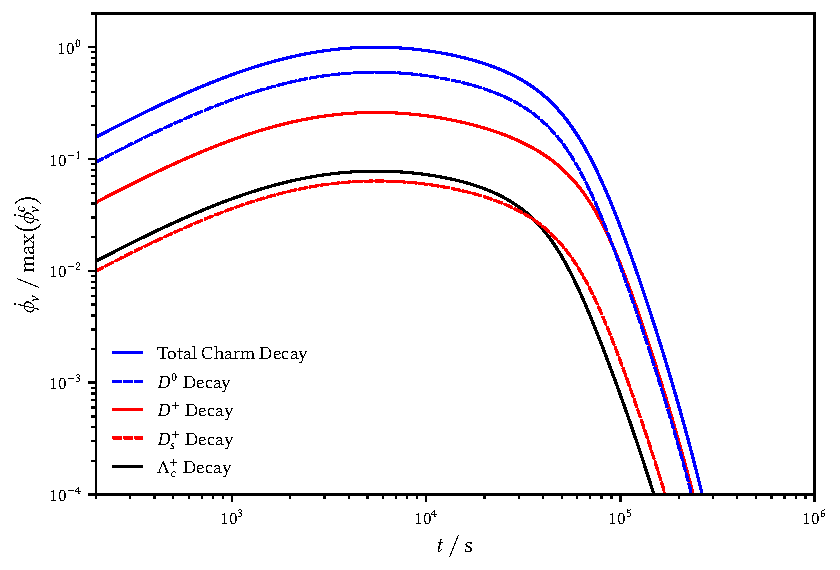
\includegraphics{../plots/build/magnetar_charm_decay_comparison_with.pdf}
	\caption[Magnetar $\nu \kern+0.5pt$ flux from $c$ decay including optical depth.]
			{Comparison of individual charmed hadron contributions to the total charm neutrino flux at
			 $E_\nu = \kern-0.5pt \qty{e9}{\giga\electronvolt}$ from a young magnetar, including the optical
			 depth defined by \eqref{eqn:optical} as a modification. Decays of $\smash{D^0}$ produce most of
			 the charmed neutrinos until later times when $\smash{D^+} \kern-0.5pt$ becomes significant, with
			 $\smash{D^+_s}$ and $\smash{\Lambda^{\kern-0.5pt +}_{\kern+0.5pt c}}$ being similar, both
			 contributing around \qty{10}{\percent} to the combined flux. This is in line with the
			 cross sections from \ref{sub:charm} as well as the branching fractions that
			 Table \ref{tab:charm-hadrons} lists.}
	\label{fig:magnetar-charm-comparison-with}
\end{figure}

\vfill\null\newpage\null\vfill
\begin{figure}[H]
	\centering
	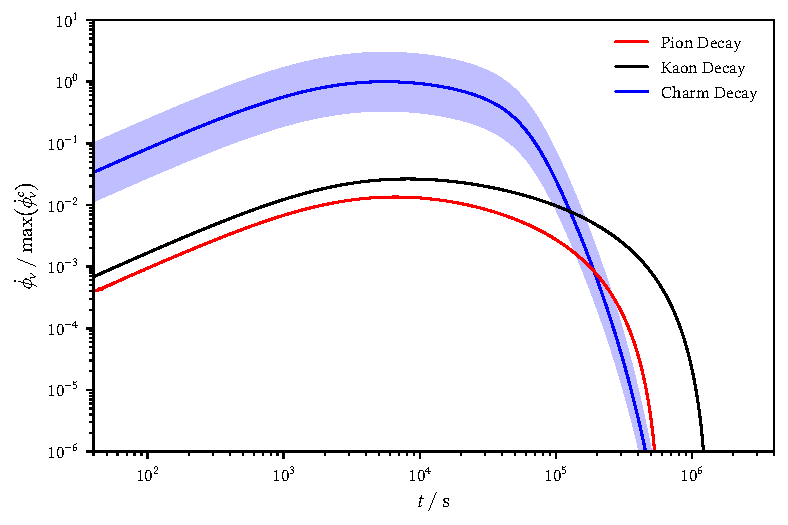
\includegraphics{../plots/build/magnetar_neutrino_spectrum_with.pdf}
	\caption[]{}
	\label{fig:magnetar-flux-with}
\end{figure}

\vfill\null\newpage\null\vfill
\begin{figure}[H]
	\centering
	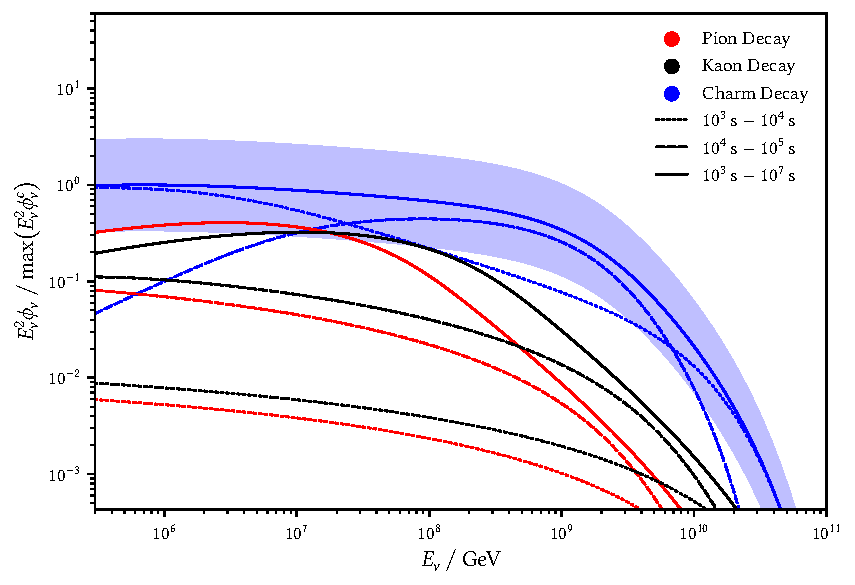
\includegraphics{../plots/build/magnetar_integrated_neutrino_spectrum_with.pdf}
	\caption[Magnetar $\nu \kern+0.5pt$ fluence compared to $c$ decay with optical depth.]
			{Expected neutrino fluence normalized to the maximum charm contribution from a~young magnetar for different time
			 intervals after formation, including the optical depth defined by \eqref{eqn:optical} as a modification.
			 Charmed hadrons dominate at all energies~except below $E_\nu = \kern-0.5pt \qty{e7}{\giga\electronvolt}$ for the
			 $\qty{e4}{\second} - \kern-1.0pt \qty{e5}{\second}$ integration. This is unexpected and therefore discussed further
			 in the text. The same shaded uncertainty band as in Figure \ref{fig:magnetar-flux-with} is adopted for charm decays.
			 Fluences are scaled by a factor $E_\nu^2$ for clarity and to facilitate the comparison to \cite{Carpio_2020}.}
	\label{fig:magnetar-fluence-with}
\end{figure}

\vfill\null\newpage

In order to evaluate the significance of different time periods, Figure \ref{fig:magnetar-fluence-with} depicts integration
results over varying intervals for pion, kaon and charm fluence. Contrary to expectations, charmed hadron decays are dominant
at all energies by as much as one order of magnitude. Comparing Figures \ref{fig:magnetar-flux-with} and
\ref{fig:magnetar-fluence-with} with the corresponding plots in \cite{Carpio_2020} reveals further inconsistencies. Notably, the
light curves in Figure \ref{fig:magnetar-flux-with} have relatively flat slopes at earlier times, and the charm neutrino fluence
in Figure \ref{fig:magnetar-fluence-with} shows no decrease at lower energies. Testing different potential error sources
indicates that the optical depth $\mathscr{O}$ is most likely responsible for these discrepancies. Inserting proportionalities
of ejecta density $\smash{n_\text{ej} \kern-0.5pt \propto t^{-3}}$ and radius $\smash{r_\text{ej} \kern-0.5pt \propto t}$ into
\eqref{eqn:optical} while assuming $\sigma_{p \kern-0.1pt p}$ to be constant leads to an approximate
$\smash{\mathscr{O} \propto t^{-2}}$ dependence and results in neutrino numbers being distorted significantly towards larger values
at earlier times. To verify this finding, calculations are repeated after omitting the optical depth.

As suspected, these results more closely match those in \cite{Carpio_2020}. Starting with the comparison of charmed hadrons, Figure
\ref{fig:magnetar-charm-comparison-without} agrees with the previous statements regarding $\smash{D^0}$ and $\smash{D^+} \kern-0.5pt$
dominating over $\smash{D^+_s}$ and $\smash{\Lambda^{\kern-0.5pt +}_{\kern+0.5pt c}}$ decays. By excluding the optical depth,
one can reveal additional information via the identification of comparatively narrow peaks. Their relative positions are consistent with
the different mean lifetimes that Table \ref{tab:charm-hadrons} lists, an observation which is not accessible from Figure
\ref{fig:magnetar-charm-comparison-with} due to flux curves resembling broad plateaus rather than clearly defined extrema. Due to shorter
decay times resulting in vanishing cooling effects \eqref{eqn:cooling} at higher energies, curves are shifted to reproduce slight offsets
in charmed hadron contribution.

Again comparing \cite{Carpio_2020} to Figures \ref{fig:magnetar-flux-without} and \ref{fig:magnetar-fluence-without} indicates improved
agreement, with distribution shapes that are roughly similar in both cases. Because of differences in the approaches, some deviation is
to be expected. Reference \cite{Carpio_2020} uses event generator results to model pion and kaon cross sections, as well as QCD calculations
for the charm component, while this thesis collects various parametrizations from the literature for semianalytical computations instead.
Especially the almost identical shapes of pion and kaon light curves in Figure \ref{fig:magnetar-flux-without} are most likely a consequence
of the simplifying assumption that their spectral distributions are linearly proportional up to a cutoff determined from their rest
masses. Despite this, neutrino fluxes from pion or kaon decay individually fit their counterparts in \cite{Carpio_2020} fairly well when
the contribution from muons is ignored, and their respective maxima are within acceptable margins compared to the charmed hadron curves in
Figure \ref{fig:magnetar-flux-without} and reference \cite{Carpio_2020}.

\newpage\null\vfill
\begin{figure}[H]
	\centering
	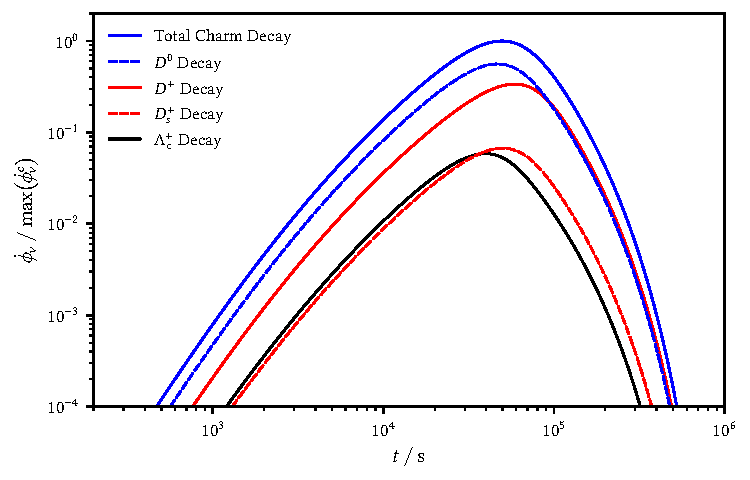
\includegraphics{../plots/build/magnetar_charm_decay_comparison_without.pdf}
	\caption[Magnetar $\nu \kern+0.5pt$ flux from $c$ decay excluding optical depth.]
			{Comparison of individual charmed hadron contributions to the total charm neutrino flux at
			 $E_\nu = \qty{e9}{\giga\electronvolt}$ from a newborn magnetar, excluding optical depth.}
	\label{fig:magnetar-charm-comparison-without}
\end{figure}

\vfill\null\newpage\null\vfill
\begin{figure}[H]
	\centering
	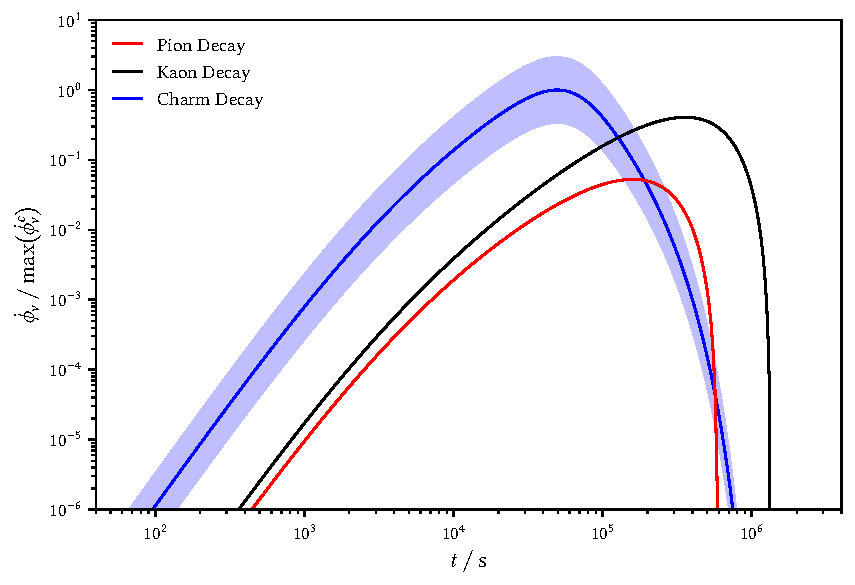
\includegraphics{../plots/build/magnetar_neutrino_spectrum_without.pdf}
	\caption[Magnetar $\nu \kern+0.5pt$ flux compared to $c$ decay without optical depth.]
			{}
	\label{fig:magnetar-flux-without}
\end{figure}

\vfill\null\newpage\null\vfill
\begin{figure}[H]
	\centering
	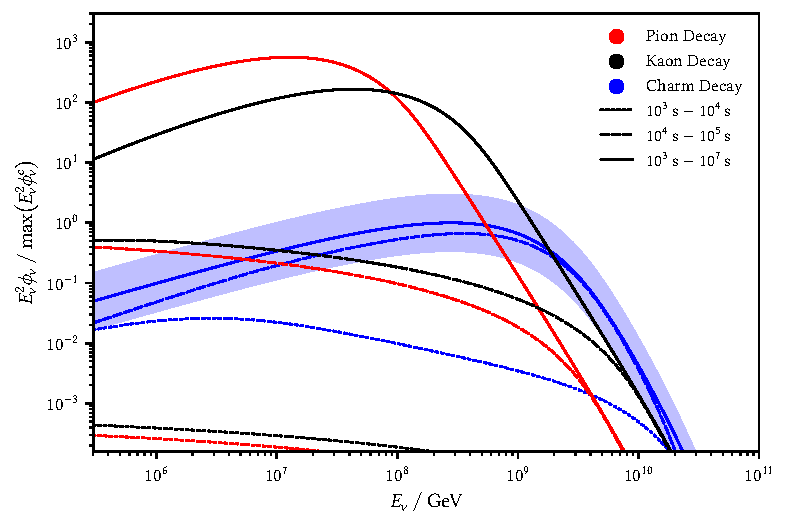
\includegraphics{../plots/build/magnetar_integrated_neutrino_spectrum_without.pdf}
	\caption[]{}
	\label{fig:magnetar-fluence-without}
\end{figure}

\vfill\null\newpage

There are, however, certain disagreements that are unlikely to arise purely from variations in the described methodologies. To begin with,
reference \cite{Carpio_2020} provides $\cramped{E^M} = \kern-0.5pt \smash{\qty{1.3e13}{\giga\electronvolt}}$ as an initial value for the
monochromatic energy of injected protons, which disagrees with the result of
$\cramped{E^M} = \kern-0.5pt \smash{\qty{1.7e12}{\giga\electronvolt}}$
obtained after inserting the same default parameters into \eqref{eqn:mono} and converting from \unit{erg} to \unit{\giga\electronvolt}
units. If the larger and seemingly erroneous value is actually used, it would imply energies one order of magnitude higher than in the
calculations presented here. Predictions from this include earlier light curve cutoffs, as energies become insufficient after less time
has passed, and potentially smaller separation between charm, pion and kaon components, because at each point in time, only lower
energy hadrons are available for neutrino production, resulting in a reduction of otherwise possible peak values. A comparison to
\cite{Carpio_2020} shows that Figure \ref{fig:magnetar-flux-without} displays both of these features. Smaller injection energies
further imply lower charm decay contributions to the total neutrino fluence, which Figure \ref{fig:magnetar-fluence-without} seems
to support as well when compared to \cite{Carpio_2020}. Adding to this concern is the large divergence from Figures
\ref{fig:magnetar-flux-with} and \ref{fig:magnetar-fluence-with} that most likely stems from the optical depth. Setting this
factor to be constant assumes a fixed fraction of protons collides to produce hadrons, independent from density changes
due to an expanding ejecta volume. Such an assumption is difficult to justify, with the potential exception
of extremely high densities. As reference \cite{Carpio_2020} explicitly includes an optical depth in the same way
this thesis does, it is unclear how the wide disparities between neutrino spectra come about, especially
considering that Figures \ref{fig:magnetar-flux-without} and \ref{fig:magnetar-fluence-without} without $\mathscr{O}$ match
better than Figures~\ref{fig:magnetar-flux-with}~and~\ref{fig:magnetar-fluence-with}~with~$\mathscr{O}$~to those in \cite{Carpio_2020}.
This issue represents a major incongruence and warrants further scrutiny, which the following chapter discusses in more detail. Due to their
agreement with prior expectations and to extract physical implications from the results, calculations without optical depth are treated as
though they were valid in the subsequent paragraphs.

Examination of Figure \ref{fig:magnetar-flux-without} confirms that charm decays exceed pion and kaon contributions at earlier times.
Peak flux values for $E_\nu = \kern-0.5pt \qty{e9}{\giga\electronvolt}$ are of similar magnitude, though pions experience stronger
suppression from cooling when compared to kaons. Inclusion of secondary muons as indicated by \cite{Carpio_2020} would
lead to increased maxima, especially for neutrinos from pion decay, but does not significantly influence the relative peak positions.
At lower energies, cooling factors approaching unity lead to pions becoming dominant, with kaons slightly below that. Neutrinos
from charmed hadrons are now suppressed due to their lower production cross sections and branching ratios. The opposite behavior
is seen as energies become larger, with contributions from charm dominating over those from pions and kaons. Light curves presented
in Figure \ref{fig:magnetar-flux-without} are shaped by cooling factors at early times when all fluxes are suppressed, increase towards
their maximum as decay and cooling timescales are equal, and subsequently decrease due to less protons being available. At later times,
as $E_p$ approaches $E_h$ and hadron production is inhibited by energy conservation, a sharp cutoff is observed in the fluxes. These
are universal characteristics, with charm, kaon and pion components being shifted with respect to each other as a result of their
different masses and lifetimes. Besides changing their magnitudes, flux curves move towards earlier times at higher energies
according to cooling and cutoff thresholds, with relative positions between individual contributions remaining mostly unaffected. 
The findings described so far are in agreement with results from \cite{Carpio_2020}.

\newpage

To evaluate the fluence, Figure \ref{fig:magnetar-fluence-without} presents different time intervals, scaled by the square of the
neutrino energy. From the flux properties follows that charm decays dominate at earlier times, followed by kaons and pions. As
the available proton energy reduces with time, each component contributes significantly at different energies, with neutrino fluence
from charmed hadrons being the most energetic. Lower energies are found for kaons, while pions comprise the lowest energy range.
In terms of the magnitudes of the neutrino fluences, pion decay up to energies around
$E_\nu = \kern-0.5pt \smash{\qty{e8}{\giga\electronvolt}}$ represents the largest contribution, beyond which kaons begin to dominate.
Significant portions of the fluence above a threshold of $E_\nu = \kern-0.5pt \smash{\qty{e9}{\giga\electronvolt}}$ originate from the
decays of charmed hadrons. The maximum proton energy imposes $E_\nu = \kern-0.5pt \smash{\qty{e12}{\giga\electronvolt}}$ as a hard cutoff,
which is not visible in Figure \ref{fig:magnetar-fluence-without} for improved readability. Contrary to what \cite{Carpio_2020} shows,
neutrinos from charm start decreasing closer to the kaon component, with kaons being approximately equal to the lower uncertainty bound
for charmed hadrons at high energies. It is therefore unclear if a charmed neutrino component is unambiguously separable from pions and
kaons. This discrepancy is at least partly attributable to the aforementioned larger maximum proton energy given in \cite{Carpio_2020}.

Continuing with results from an AGN accretion disk, there exists no temporal dimension, as the model
assumes a constant neutrino spectrum at first approximation. Depicted in Figure \ref{fig:nucleus-charm-comparison}
are the individual charmed hadron contributions to the total charm fluence, again with a scaling of neutrino energy squared.
This agrees well with findings for the magnetar setting, as decays of both $\smash{D^0}$ and $\smash{D^+} \kern-0.5pt$ dominate
over $\smash{D^+_s}$ and $\smash{\Lambda^{\kern-0.5pt +}_{\kern+0.5pt c}}$ components at all energies. Thanks to its larger
branching fraction, contribution from $\smash{D^+} \kern-0.5pt$ slightly exceeds $\smash{D^0}$ up to
$E_\nu = \kern-0.5pt \qty{e9}{\giga\electronvolt}$ despite having a smaller production cross section \cite{lhc}. At higher energies,
the longer lifetime for $\smash{D^+}$ listed in Table \ref{tab:charm-hadrons} leads to suppression via cooling, leaving $\smash{D^0}$
as the dominant charm contributor.

The combined charm fluence is presented by Figure \ref{fig:nucleus-fluence} with neutrinos from pion and kaon decay. All curves have
shapes roughly similar to those in Figure \ref{fig:magnetar-fluence-without} for the magnetar scenario, with a slow rise at lower
energies and a downward slope from cooling in higher energy ranges. The flat regions for pions and kaons are not visible in Figure
\ref{fig:nucleus-fluence} due to their longer lifetimes. Additionally, kaon decay surpasses the pion component at all included energies,
though this changes towards lower energy values that are, however, excluded from the view in order to highlight charmed hadrons. Neutrino
fluence from charm is dominant from $E_\nu = \kern-0.5pt \qty{e9}{\giga\electronvolt}$~and decreases at energies of
$E_\nu = \kern-0.5pt \qty{e10}{\giga\electronvolt}$ and above. This agrees with expectations from cooling effects and is sensitive
to the chosen density, as larger values lead to a considerable reduction of the threshold energy. From its gradual slope up to the
maximum charm fluence, one can infer a power law as the underlying proton spectrum, which is only slightly modified through the optical
depth including a cross section \eqref{eqn:hpr1r2} that slowly increases with energy. These results further account for decays occurring
after hadrons have passed through the accretion disk by checking if decay distances exceed the scale height and setting an according
cooling factor, although no significant effects on the contributions are observed by including this step.

A major limitation applying to all findings of this thesis concerns the employed parametrizations. Chapter \ref{ch:methods}
clarifies how these are collected from various sources and combined by using several simplifying assumptions, which potentially
introduce errors that are larger than anticipated. As discussed below, this may be resolved by directly using data from event
generators, which track hadronic interactions based on parton models.

\enlargethispage*{\baselineskip}\newpage\null\vfill
\begin{figure}[H]
	\centering
	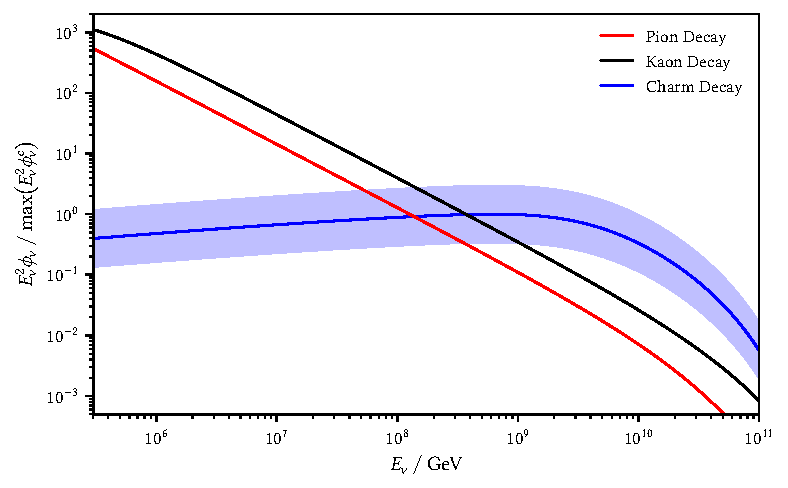
\includegraphics{../plots/build/nucleus_neutrino_spectrum.pdf}
	\caption[AGN accretion disk $\nu \kern+0.5pt$ fluence compared to $c$ decay.]
			{}
	\label{fig:nucleus-fluence}
\end{figure}

\vfill\null\newpage\null\vfill
\begin{figure}[H]
	\centering
	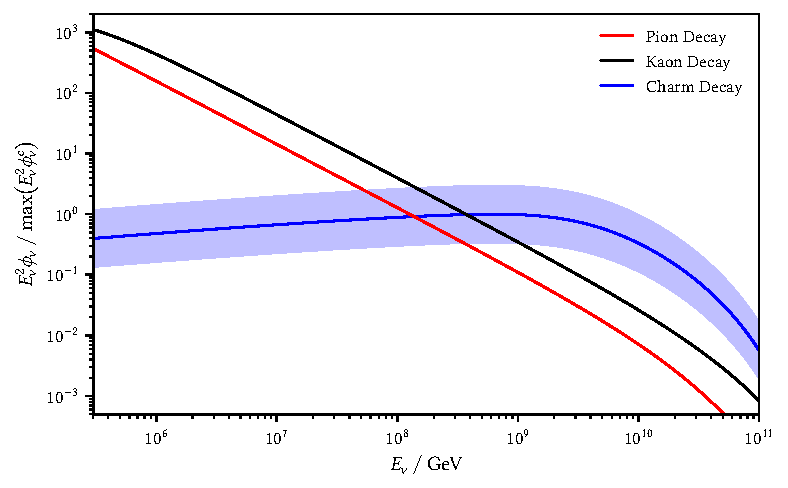
\includegraphics{../plots/build/nucleus_neutrino_spectrum.pdf}
	\caption[AGN accretion disk $\nu \kern+0.5pt$ fluence compared to $c$ decay.]
			{Expected neutrino fluence normalized to the maximum charmed hadron contribution from an AGN accretion disk.
			 Differences between the shapes of pion and kaon components compared to charm decays result from the chosen
			 view, as the flat increase observed for charmed hadrons occurs at lower energies in the case of pions and kaons
			 due to their much longer lifetimes. These decay times are listed in Sections \ref{sub:scattering} and \ref{sub:charm}
			 with Figure \ref{fig:nucleus-charm-comparison} giving the reasoning for effects of cooling. Charmed hadrons dominate
			 the fluence from $E_\nu = \kern-0.5pt \qty{e9}{\giga\electronvolt}$ and above, lining up with prior expectations. This
			 threshold is sensitive to varying densities, with lower values producing a shift towards higher energies. A hard cutoff
			 is enforced by $E_p = \kern-0.5pt \qty{e12}{\giga\electronvolt}$ as the maximum proton energy. The same shaded uncertainty
			 band as in Figure \ref{fig:magnetar-flux-with} for charm decays as well as the scaling by $E_\nu^2$ from
			 Figure \ref{fig:magnetar-fluence-with} are adopted.}
	\label{fig:nucleus-fluence}
\end{figure}

\vfill\null\newpage
